%%%%%%%%%%%%%%%%%%%%%%%%%%%%%%%%%%%%%%%%%
% Daily Laboratory Book
% LaTeX Template 
%
% This template has been downloaded from:
% http://www.latextemplates.com
%
% Original author:
% Frank Kuster (http://www.ctan.org/tex-archive/macros/latex/contrib/labbook/)
%
% Important note:
% This template requires the labbook.cls file to be in the same directory as the
% .tex file. The labbook.cls file provides the necessary structure to create the
% lab book.
%  %%mikeg: Since labbook is installed shouldn't need to do this
% The \lipsum[#] commands throughout this template generate dummy text
% to fill the template out. These commands should all be removed when 
% writing lab book content.
%
% HOW TO USE THIS TEMPLATE 
% Each day in the lab consists of three main things:
%
% 1. LABDAY: The first thing to put is the \labday{} command with a date in 
% curly brackets, this will make a new page and put the date in big letters 
% at the top.
%
% 2. EXPERIMENT: Next you need to specify what experiment(s) you are 
% working on with an \experiment{} command with the experiment shorthand 
% in the curly brackets. The experiment shorthand is defined in the 
% 'DEFINITION OF EXPERIMENTS' section below, this means you can 
% say \experiment{pcr} and the actual text written to the PDF will be what 
% you set the 'pcr' experiment to be. If the experiment is a one off, you can 
% just write it in the bracket without creating a shorthand. Note: if you don't 
% want to have an experiment, just leave this out and it won't be printed.
%
% 3. CONTENT: Following the experiment is the content, i.e. what progress 
% you made on the experiment that day.
%
%%%%%%%%%%%%%%%%%%%%%%%%%%%%%%%%%%%%%%%%%
\documentclass[letterpaper,index=totoc,hyperref,openany]{labbook} % 'openany' here removes the gap page between days, erase it to restore this gap; 'oneside' can also be added to remove the shift that odd pages have to the right for easier reading

%----------------------------------------------------------------------------------------
%	PACKAGES AND OTHER DOCUMENT CONFIGURATIONS
%----------------------------------------------------------------------------------------

\usepackage[ 
%  backref=page, %incompatible with biblatex
  pdfpagelabels=true,
  plainpages=false,
  colorlinks=true,
  bookmarks=true,
  pdfview=FitB]{hyperref} % Required for the hyperlinks within the PDF
  
\usepackage{booktabs} % Required for the top and bottom rules in the table
\usepackage{float} % Required for specifying the exact location of a figure or table
\usepackage{graphicx} % Required for including images

%%Customizations by mikeg
\usepackage{marginnote}%provides ability to put notes in the margin using \marginnote{} coommand
\usepackage{ifthen}
\usepackage{amsmath,amssymb}
\usepackage{xspace}
\usepackage{listings} %provides lstlisting environment for typesetting code
\usepackage[natbib=true,backref=page]{biblatex} %alternative to natbib

\bibliography{/home/mikeg/BiBTeX/bibliography.full}

\usepackage{etoolbox}
\makeatletter
%suppress pagebreaks between days
\patchcmd{\addchap}{\if@openright\cleardoublepage\else\clearpage\fi}{\par}{}{}
%\patchcmd{\scr@startchapter}{\if@openright\cleardoublepage\else\clearpage\fi}{}{}{}
%remove numbering of experiments
%\renewcommand*\theexperiment{}
%\renewcommand*\thesubexperiment{}
\makeatother 

\newcommand{\HRule}{\rule{\linewidth}{0.5mm}} % Command to make the lines in the title page
\setlength\parindent{0pt} % Removes all indentation from paragraphs


%----------------------------------------------------------------------------------------
%	TITLE PAGE
%----------------------------------------------------------------------------------------
\begin{document}
\frontmatter % Use Roman numerals for page numbers
\title{Undergraduate Research Assistant Notes}
\begin{center}
\HRule \\[0.4cm]
{\Huge \bfseries Research Journal \\[0.4cm] % Degree
\HRule \\[1.5cm]}
\end{center}

\author{\LARGE Walker Bussey-Spencer \\ \Large wbusseys@vols.utk.edu \\[2cm]} % Your name and email address
\date{Beginning 22 July 2016} % Beginning date



%\newexperiment{<abbrev>}[<short form>]{<long form>}
%Here, <abbrev> is the abbreviation that can be given later to make LATEX
%use the <long form> and <short form>. The short form is for index, table of
%contents and running title, and giving it is optional. When using the abbre-
%viation, specify it without prepending a backslash, i.e. \experiment{abbrev}.
%Abbreviations may contain any char except the backslash, the tilde ( ̃), comma

\newexperiment{NSE}{NSE SEMPPR}
\newexperiment{ROC}{ROC SEMPPR}
\newexperiment{RPF-ROC}[RPF-ROC]{Ribosome Profile Footprints: Pausing Model}
\newexperiment{RPF-NSE}[RPF-NSE \& ROC]{Ribosome Profile Footprints: NSE \& Pausing Model}
\newexperiment{FONSE}{FONSE SEMPPR}
\newexperiment{DIMCMC}[DIMCMC]{Doubly Intractable MCMC}
\newexperiment{Knight}{Student Learning, Jennifer Knight}
\newexperiment{SELAC}{Main SELAC model}
\newexperiment{Lab}{Lab Meeting}
\newexperiment{LSAs}{LSAs}
\newexperiment{Cedric}{Cedric Landerer}
\newexperiment{Mehmet}{Mehmet Aydeniz}
\newexperiment{SMBE Satellite Meeting on Protein Evolution in Denver}{SMBEDen}
%\newexperiment{shorthand}{Description of the experiment}


%COMMANDS
%%% Sort using M-x 'sort-lines'
\newcommand{\GTR}{GTR+$\Gamma$\xspace}
\newcommand{\LogN}{\ensuremath{\text{LogN}}\xspace}
\newcommand{\Lik}{\ensuremath{\text{\textbf{Lik}}}\xspace}
\newcommand{\LLik}{\ensuremath{\mathcal{L}}\xspace}
\newcommand{\Ne}{\ensuremath{{N_e}}\xspace}
\newcommand{\Piihat}{\ensuremath{\hat{\pi}_i}\xspace}
\newcommand{\Pii}{\ensuremath{\pi_{i}}\xspace}
\newcommand{\Pijhat}{\ensuremath{\hat{\pi}_j}\xspace}
\newcommand{\Pij}{\ensuremath{\pi_{j}}\xspace}
\newcommand{\Pivechat}{\ensuremath{\hat{\Pivec}}\xspace}
\newcommand{\Pivec}{\ensuremath{\Vec{\pi}}\xspace}
%\newcommand{\Pr}{\ensuremath{\text{Pr}}\xspace}
\newcommand{\Qmatrixa}{\ensuremath{\Qmatrix_a}\xspace}
\newcommand{\Qmatrix}{\mathbf{Q}\xspace}
\newcommand{\ROC}{\ensuremath{\text{ROC}}\xspace}
\newcommand{\Var}{\operatorname{Var}}
\newcommand{\var}{\Var}
\newcommand{\Wi}{\ensuremath{{W_i}}\xspace}
\newcommand{\Wj}{\ensuremath{{W_j}}\xspace}
\newcommand{\acivec}{\ensuremath{a\left(\cveci\right)}\xspace}
\newcommand{\acvecg}{\ensuremath{a\left(\vec{c}_{i,g}\right)}\xspace}
\newcommand{\acvecj}{\ensuremath{a\left(\cvecj\right)}\xspace}
\newcommand{\acvec}{\ensuremath{a\left(\Vec{c}\right)}\xspace}
\newcommand{\aip}{\ensuremath{a_{i,p}}\xspace}
\newcommand{\aivecg}{\ensuremath{{\avec}_{i,g}}\xspace}
\newcommand{\aivec}{\aveci}
\newcommand{\ajp}{\ensuremath{a_{j,p}}\xspace}
\newcommand{\ajvecg}{\ensuremath{{\ajvec}_{,g}}\xspace}
\newcommand{\ajvec}{\ensuremath{\Vec{a}_{j}}\xspace}
\newcommand{\aj}{\ensuremath{a__j}\xspace}
\newcommand{\alphac}{\ensuremath{\alpha_c}\xspace}
\newcommand{\alphap}{\ensuremath{\alpha_p}\xspace}
\newcommand{\alphavec}{\ensuremath{\Vec{\alpha}}\xspace}
\newcommand{\alphav}{\ensuremath{\alpha_v}\xspace}
\newcommand{\aobsvecg}{\ensuremath{{\avec}_{\text{obs},g}}\xspace}
\newcommand{\aobsvec}{\ensuremath{\Vec{a}_{\text{obs}}}\xspace}
\newcommand{\aobs}{\ensuremath{a_{\text{obs}}}\xspace}
\newcommand{\aoptip}{\ensuremath{\aopt_{i,p}}\xspace}
\newcommand{\aoptpg}{\ensuremath{\aopt_{p,g}}\xspace}
\newcommand{\aoptp}{\ensuremath{\aopt_p}\xspace}
\newcommand{\aoptvecg}{\ensuremath{{{\aoptvec}_g}}\xspace}
\newcommand{\aoptvec}{\ensuremath{\Vec{a}^*}\xspace}
\newcommand{\aopt}{\ensuremath{{a^*}}\xspace}
\newcommand{\aveci}{\ensuremath{\Vec{a}_i}\xspace}
\newcommand{\avecj}{\ensuremath{\Vec{a}_j}\xspace}
\newcommand{\avec}{\ensuremath{\Vec{a}}\xspace}
\newcommand{\avecopt}{\aoptvec}
\newcommand{\celegans}{\emph{C.~elegans}\xspace}
\newcommand{\cveci}{\ensuremath{\cvec_i}\xspace}
\newcommand{\cvecj}{\ensuremath{\cvec_j}\xspace}
\newcommand{\cvec}{\ensuremath{\Vec{c}}\xspace}
\newcommand{\deltaT}{\ensuremath{\delta t}\xspace}
\newcommand{\ecoli}{\emph{E.~coli}\xspace}
\newcommand{\Lklu}{\emph{L.~kluyveri}\xspace}
\newcommand{\bsubtilis}{\emph{B.~subtilis}\xspace}
\newcommand{\fij}{\ensuremath{f_{i,j}}\xspace}
\newcommand{\gen}{\ensuremath{\text{gen}}\xspace}
\newcommand{\jmax}{\ensuremath{{j_{\max}}}\xspace}
\newcommand{\kmax}{\ensuremath{{k_{\max}}}\xspace}
\newcommand{\muij}{\ensuremath{\mu_{i,j}}\xspace}
\newcommand{\phiROC}{\ensuremath{\phi_\ROC}\xspace}
\newcommand{\phig}{\ensuremath{\phi_{g}}\xspace}
\newcommand{\pij}{\ensuremath{p_{i,j}}\xspace}
\newcommand{\qij}{\ensuremath{q_{i,j}}\xspace}
\newcommand{\qji}{\ensuremath{q_{i,j}}\xspace}
\newcommand{\rib}{\ensuremath{\text{rib}}\xspace}
\newcommand{\cell}{\ensuremath{\text{cell}}\xspace}
\newcommand{\sphi}{\ensuremath{s_\phi}\xspace}
\newcommand{\scer}{\emph{S.~cerevisiae}\xspace}
\newcommand{\setG}{\ensuremath{\mathbb{G}}\xspace}
\newcommand{\setP}{\ensuremath{\mathbb{P}}\xspace}
\newcommand{\setC}{\ensuremath{\mathbb{C}}\xspace}
\newcommand{\setF}{\ensuremath{\mathbb{F}}\xspace}
\renewcommand{\ng}{\ensuremath{{n_g}}\xspace}
\newcommand{\researcher}{\subsubsection}
%---------------------------------------------------------------------------------------

\graphicspath{{./Figures//}} % double slash indicates search recursively within folder
%%Figures will be organized in subfolders by year/month
\DeclareGraphicsExtensions{.pdf, .png, .jpg} %prevent the need for using file extensions



\frontmatter

\maketitle

\tableofcontents

\mainmatter % Use Arabic numerals for page numbers

%----------------------------------------------------------------------------------------
%	LAB BOOK CONTENTS
%----------------------------------------------------------------------------------------

% Blank template to use for new days:

%\labday{Day, Date Month \Year}

%\experiment{}

%Text

%-----------------------------------------

%\experiment{}

%\begin{figure}[H] % Example of including images
%\begin{center}
%\includegraphics[width=0.5\linewidth]{example_figure}
%\end{center}
%\caption{Example figure.}
%\label{fig:example_figure}
%\end{figure}

%Text

%----------------------------------------------------------------------------------------
%each sentence gets its own line!

%How to push/pull with git:

%git status is useful to make sure everything's right
%How to push to git repository
%git pull
%git add .
%git commit -m "July 24 note update"
%git push

%Always run pdf latex from folder containing Wnotes.tex
%----------------------------------------------------------------------------------


\labday{22 July 2016}
\experiment{C. Elegans Life Stages}
\researcher{Walker Bussey-Spencer}
\begin{itemize}
  \item Looking at data with original model— accounting for noise and include an intercept
  \item Created 2 non-overlapping sets out of the life stages
    \begin{itemize}
	\item First set includes more data points and is called “lower hierarchy” 
	\item Second set includes fewer, more encompassing data points and is called “higher hierarchy”
    \end{itemize}
  \item Running the MCMC with each of these different selected data sets.
  \end{itemize}


\begin{itemize}
\item Meeting with Dr. Gilchrist:
\item On the far right of Figure 1 we derived the weighting coefficient/expression coefficient omega as a function of time and ATP cost importance.
\item Then, to handle the fact that we do not necessarily know the length of time stages or the definite occurrence of each time stage, we defined omega in terms of the probability of observing a given time stage for a certain amount of time divided by the total proabability.
\item There was also a factor of the cost importance in the particular stage compared to probably the overall cost importance.
\item We established that the probability of observing a certain life stage was = 1 for the life stages which are inevitable for the C. Elegans, specifically: the embryonic stages, L1, L4, and Adult stage.
\item The probability of observing dauer, l2 dauer, and post dauer were all equal, and also were equal to 1 - probability of entering L2/L3.
\item The last formula we arrived at was that the probability of a life stage is equal to the the product of the omega, the total time, and the average ATP cost divided by the product of the expected value of the time in the life stage and the life stage specific q value.
\item Since we know the expected time value and the omega value, we can obtain ratio values for the different q values, as the total time and average q can cancel out.
\item We also can look at the assumption that the embryonic stages all have the same relative q values since there is a limited amount of energy in the egg that does not change in a ratio between life stages.
\item The first step now is to write two codes that include all the dauer stages and differ only in the accounting for the two aforementioned non-overlapping sets.
\item To Do:
\begin{itemize}
\item Address how the measurements in a stage that consists of substages is generated.
\item Find out where Cedric got the data.
\item Look at how the mass of the worm changes with each life stage to gain insight into the q values.
\item Make sure sum of weighting constraints = 1.
\item Write the code for each set.
\end {itemize}
\end{itemize}

\begin{figure}[H]
\begin{center}
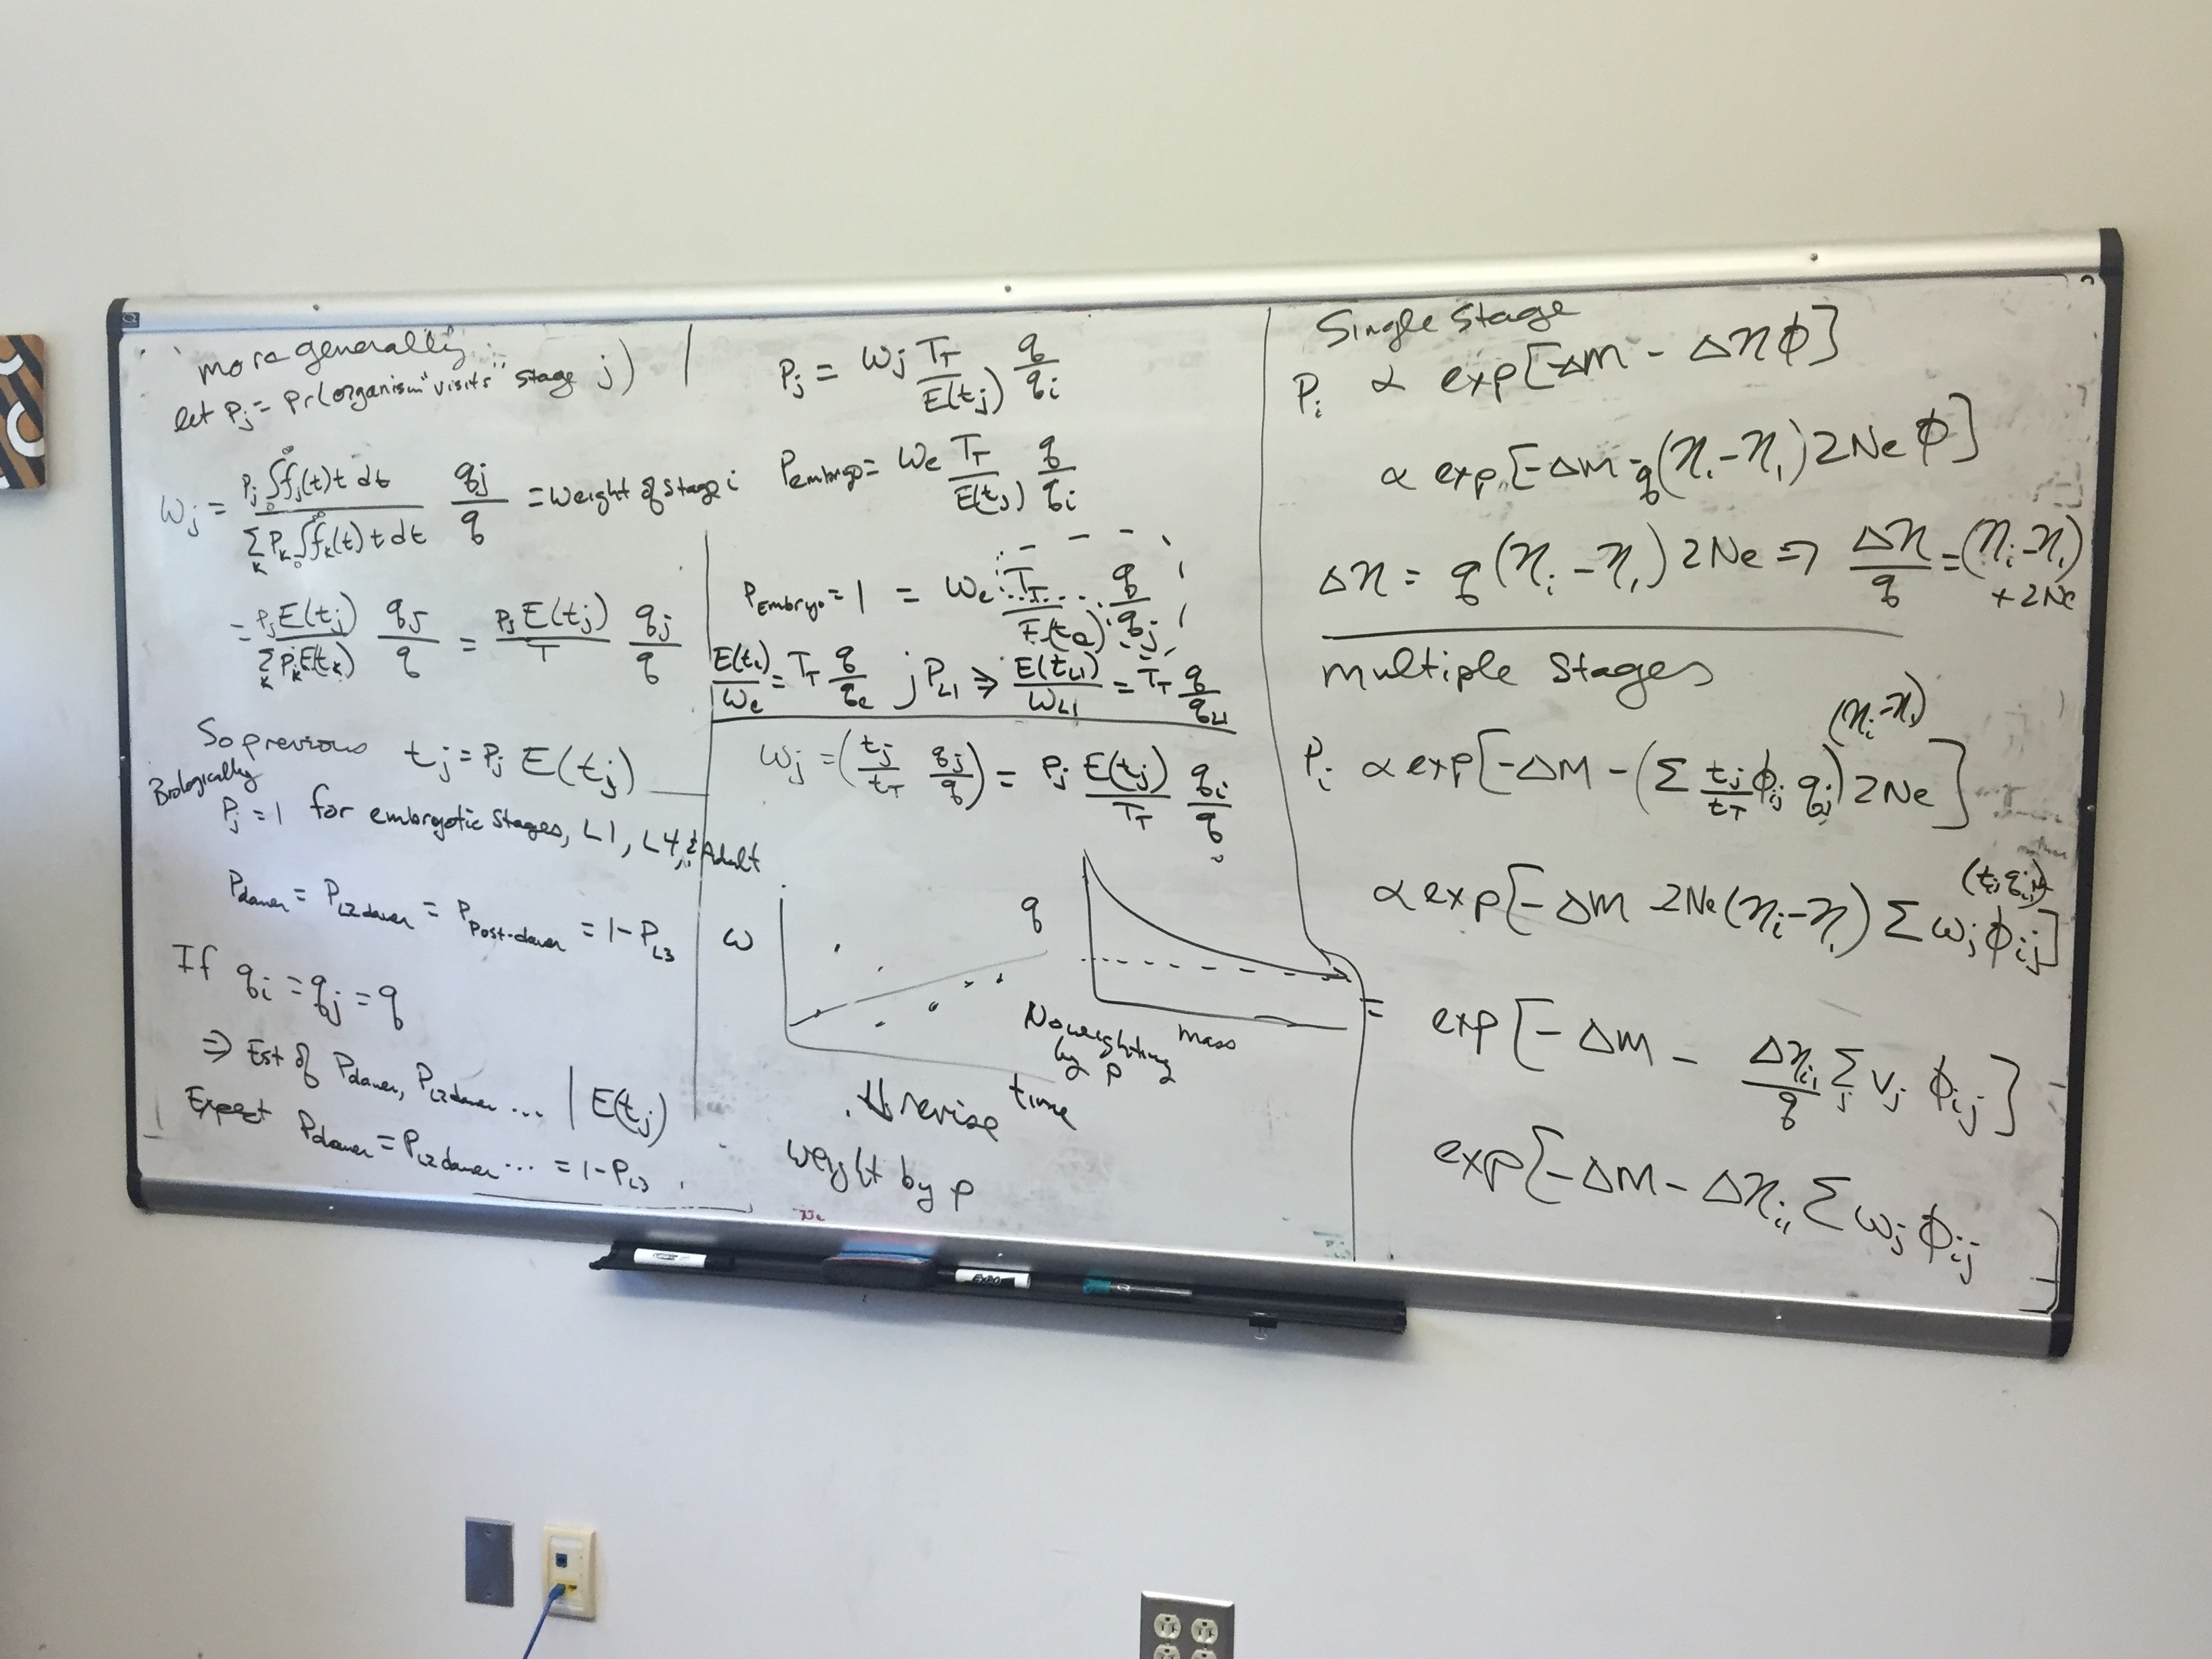
\includegraphics[scale=.1]{../Figures/2016/July_22/OmegaDerivation.jpg}
\end{center}
\caption{July 22nd Derivation of Expression Coefficient as a Multivariable Function}
\end{figure}

\labday{25 July 2016}
\experiment{C. Elegans Life Stages}
\begin{itemize}
\item Morning Meeting:
\begin{itemize}
\item Look up what unit testing is.
\item Look up mortality Leslie matrix.
\item Look up Hawk and Dove game.
\end{itemize}
\item Trying to gain comfort and ability with this latex program and to become more adept at making notes.
\item Asked Cedric where he got the life stages data and he gave me the link to the website:
\item https://www.ebi.ac.uk/gxa/experiments/E-MTAB-2812
\item Will try to type up the mathematics tomorrow.
\end{itemize}

\labday{26 July 2016}
\experiment{C. Elegans Life Stages}
\begin{itemize}
\item Finished making code for both the higher nonoverlapping set with Dauer and the lower nonoverlapping set with Dauer both allow for an intercept $ \alpha$ term.
\begin{itemize}
\item Lower includes: 4-cell, gastrulating, enclosing, 3-fold, fully-elongated, L1, L2, L3, L4, adult, L2D, Dauer, Post-Dauer.
\item Higher includes: proliferating, elongating, fully-elongated, L1, L2, L3, L4, adult, L2D, Dauer, Post-Dauer.
\end{itemize}
\item Running the Model currently.
\item Looking into how the Empirical Life Stage Data was obtained.
\item Name of the Experiment we got the data from: E-MTAB-2812 - Deep sequencing of the Caenorhabditis elegans transcriptome using RNA isolated from various developmental stages under various experimental conditions RW0001 - uninfected worms.
\item Does it matter that the data comes from various strains?
\item There is a slight variation in the different type of cells that each run looked at.
\item Although most give the cell type as organism, there is also some data taken from specifically somatic cells and neuronal motor cells.
\begin{itemize}
\item These different cell types have very different 
\item The study also includes varying ages for some of their life stages.
\begin{itemize}
\item 3-fold Embryo has 12 runs that have ages ranging from 500-710 minutes old, but each run consists of a 150 minute span.
\item Elongating Embryo has 15 runs that have ages ranging from 350-620 minutes old, but each run consists of a 150 minute span.
\item Enclosing Embryo has 5 runs that have ages ranging from 170-350 minutes old with each run consisting of a 150 minute span.
\item Fully Elongated Embryo has 17 runs, 9 of which do not have ages provided, with the other 8 ranging from 590-830 minutes and each spanning 150 minutes.
\item Gastrulating Embryo has 6 runs, 1 of which does not have an age provided, with the other 5 ranging from 80-300 minutes old, and all but one spanning 190 minutes each but the exception spans 150 minutes.
\item Late Cleavage has 7 runs that range from 230-470 minutes old, each spanning 150 minutes.
\item Proliferating Embryo has 28 runs, but only 14 runs have ages provided. These ages range from 0 - 200 minutes with each spanning 150 minutes.
\item There is no age data provided for the runs of 4-Cell Embryo, Adult, Dauer, Embryo, L1, L2, L3, L4, L2D-dauer, Post-Dauer.
\item Total of 201 runs analyzed.
\end{itemize}
\item Analysis Methods: (Directly Quoted)
\item Pipeline Version: iRAP 0.6.1p9
\item Analyzed Libraries: Single-end only
\item Filtering Steps: 
\begin{itemize}
\item Step 1- Discard reads below minimum quality threshold.
\item Step 2- Check of bacterial contamination; discard offending reads.
\item Step 3- Discard reads with common uncalled characters (e.g. N)
\item Step 4- Remove reads from pair-end libraries that were orphaned by filtering steps 1-3.
\end{itemize}
\item Read Mapping: Against genome reference (Ensembl Metazoa release: 26) tophat2 version: 2.0.12
\item Quantification: htseq2 version: 0.6.1p1
\item Normalized Counts Per Gene: 
\begin{itemize}
\item (FPKMs) are calculated from the raw counts by iRAP. 
\item These are averaged for each set of technical replicates, and then quantile normalized within each set of biological replicates using limma. 
\item Finally, they are averaged for all biological replicates (if any)
\end{itemize}
\item Model finished running and I have the results located in files that I will push to github.
\item I will run the other model tonight as it would be interrupted by my shutting my computer when I leave later.
\item TO DO:
\item Run Model with other set of data.
\item Continue to research about the empirical data.
\item Start writing code to compare the results.
\end{itemize}
\end{itemize}

\labday{27 July 2016}
\experiment{C. Elegans}
\begin{itemize}
\item I ran the model for the higher hierarchy with dauer included last night and recorded the results in the file \enquote{Model\_Results\_Higher\_With\_Dauer}.
\item The results from yesterday's run of the lower hierarchy with dauer are in the file \enquote{Model\_Results\_Lowest\_With\_Dauer}.
\item The mean log likelihood for the higher hierarchy with dauer was -57252.98 while the mean log likelihood for the lower hierarchy with dauer was -49394.46.
\item In these two files I have the mean value for each weighting coefficients--called beta in the file--and the values of the 2.5\% and 97.5\% quantiles.
\item *** Would overlapping gene use in different life stages affect the weighting and artificially increase or decrease the values in life stages that show similar transcription activity?... e.g. proliferating.. 
\item I would assume that all the cell activity is similar throughout the replication processes in each of the proliferating stages. 
\item Getting an expected time equal to the full time of proliferation for the 4-cell stage is a hypothesis in the lower hierarchy.
\item I further catalogued all of the ages given by the experiment into the same excel file that has the original life stage and order numbers.
\item That file name is \enquote{C\_Elegans/Data/Ordered.Time.Spent.Lifestages.Celeg\_1.csv}.
\item Below I will attach two PDFs that have the graphic results from each trial run.
\end{itemize}

\begin{figure}[H]
\begin{center}
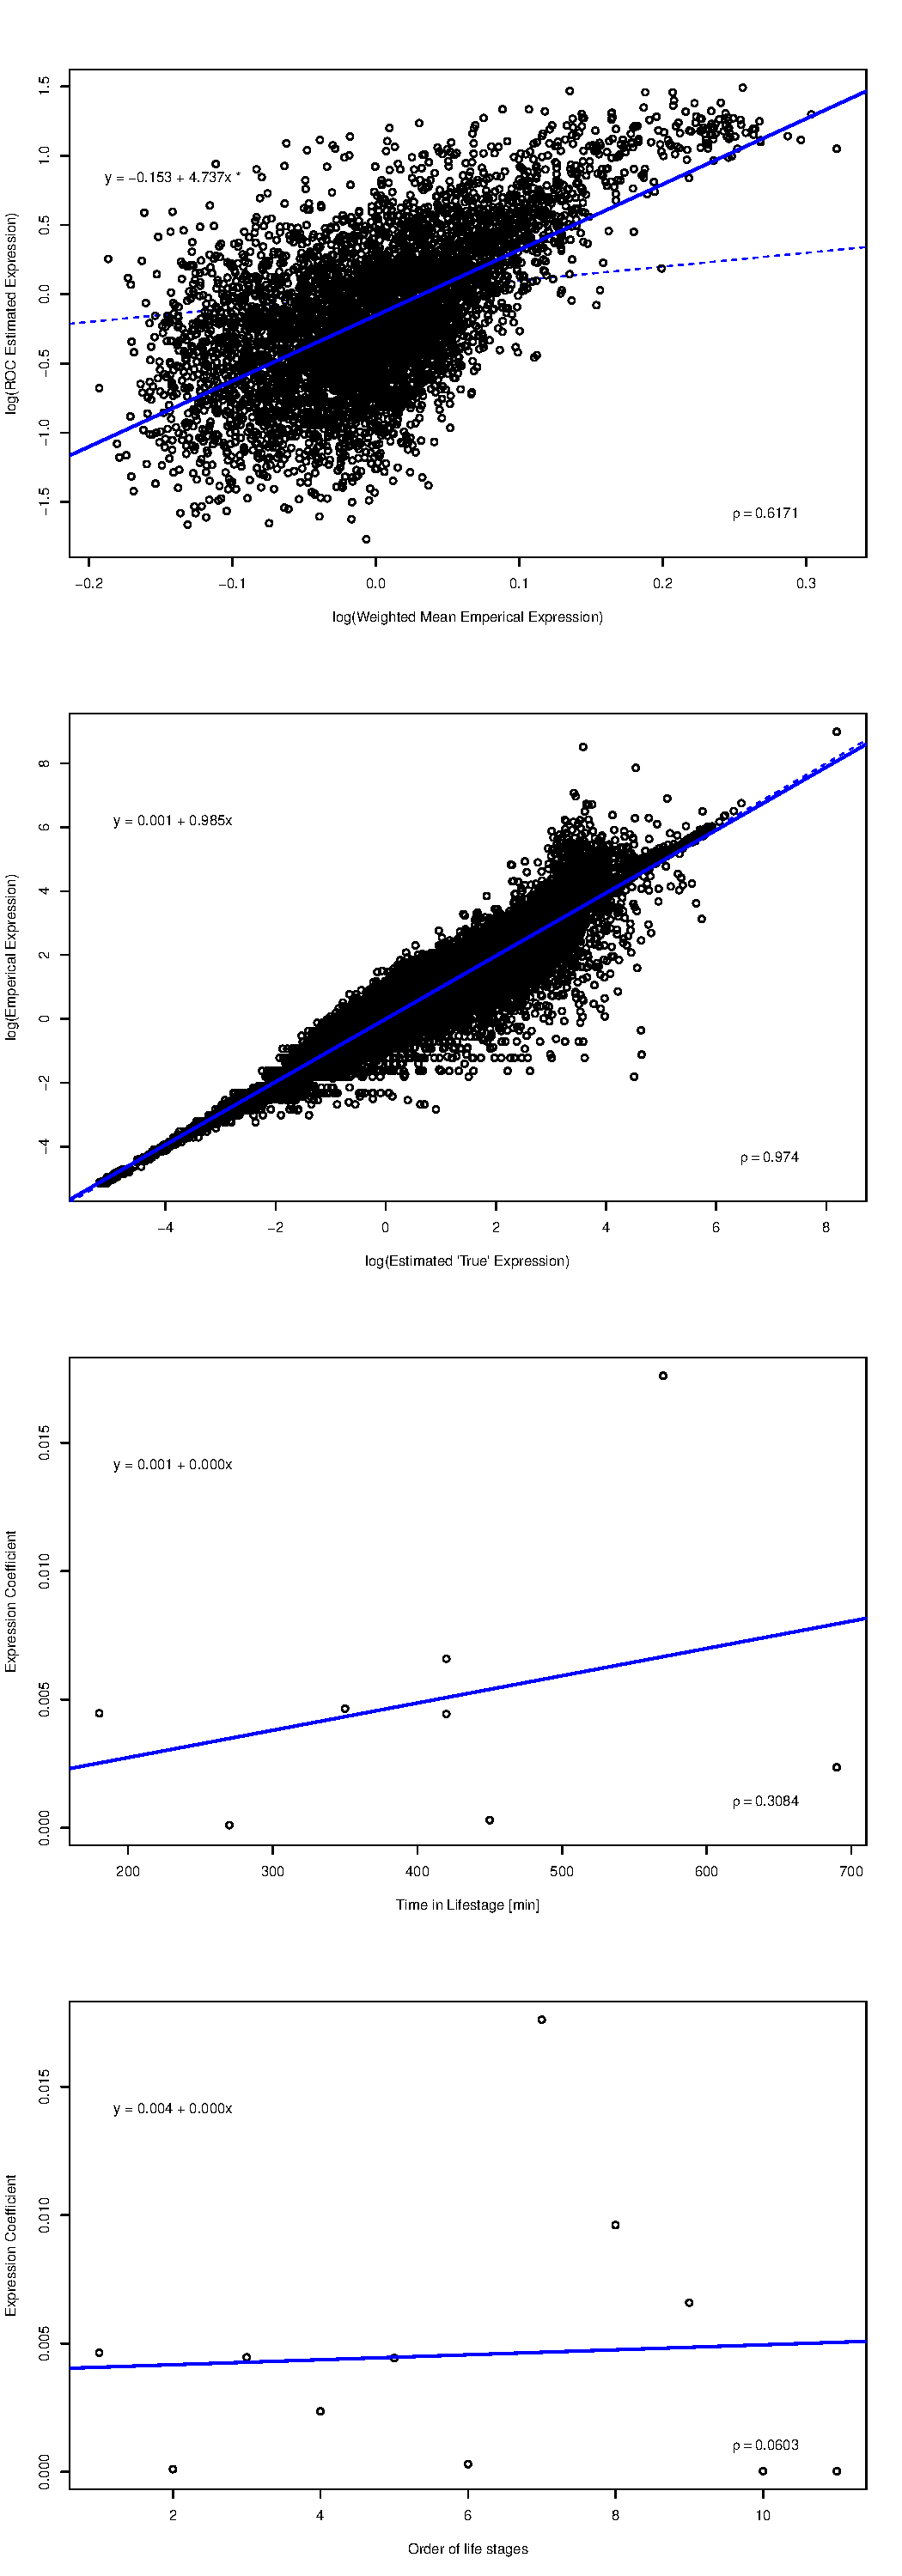
\includegraphics[scale=.45]{../C_Elegans/Higher_Hierarchy_with_Dauer_1/Plots/Higher_hierarchy_with_dauer_original_model_celegans_weighted_expr_vector_beta_noise_fixed_sroc_withIntercept.pdf}
\end{center}
\caption{July 27th Graphs From Higher Hierarchy With Dauer Model Run}
\end{figure}

\begin{figure}[H]
\begin{center}
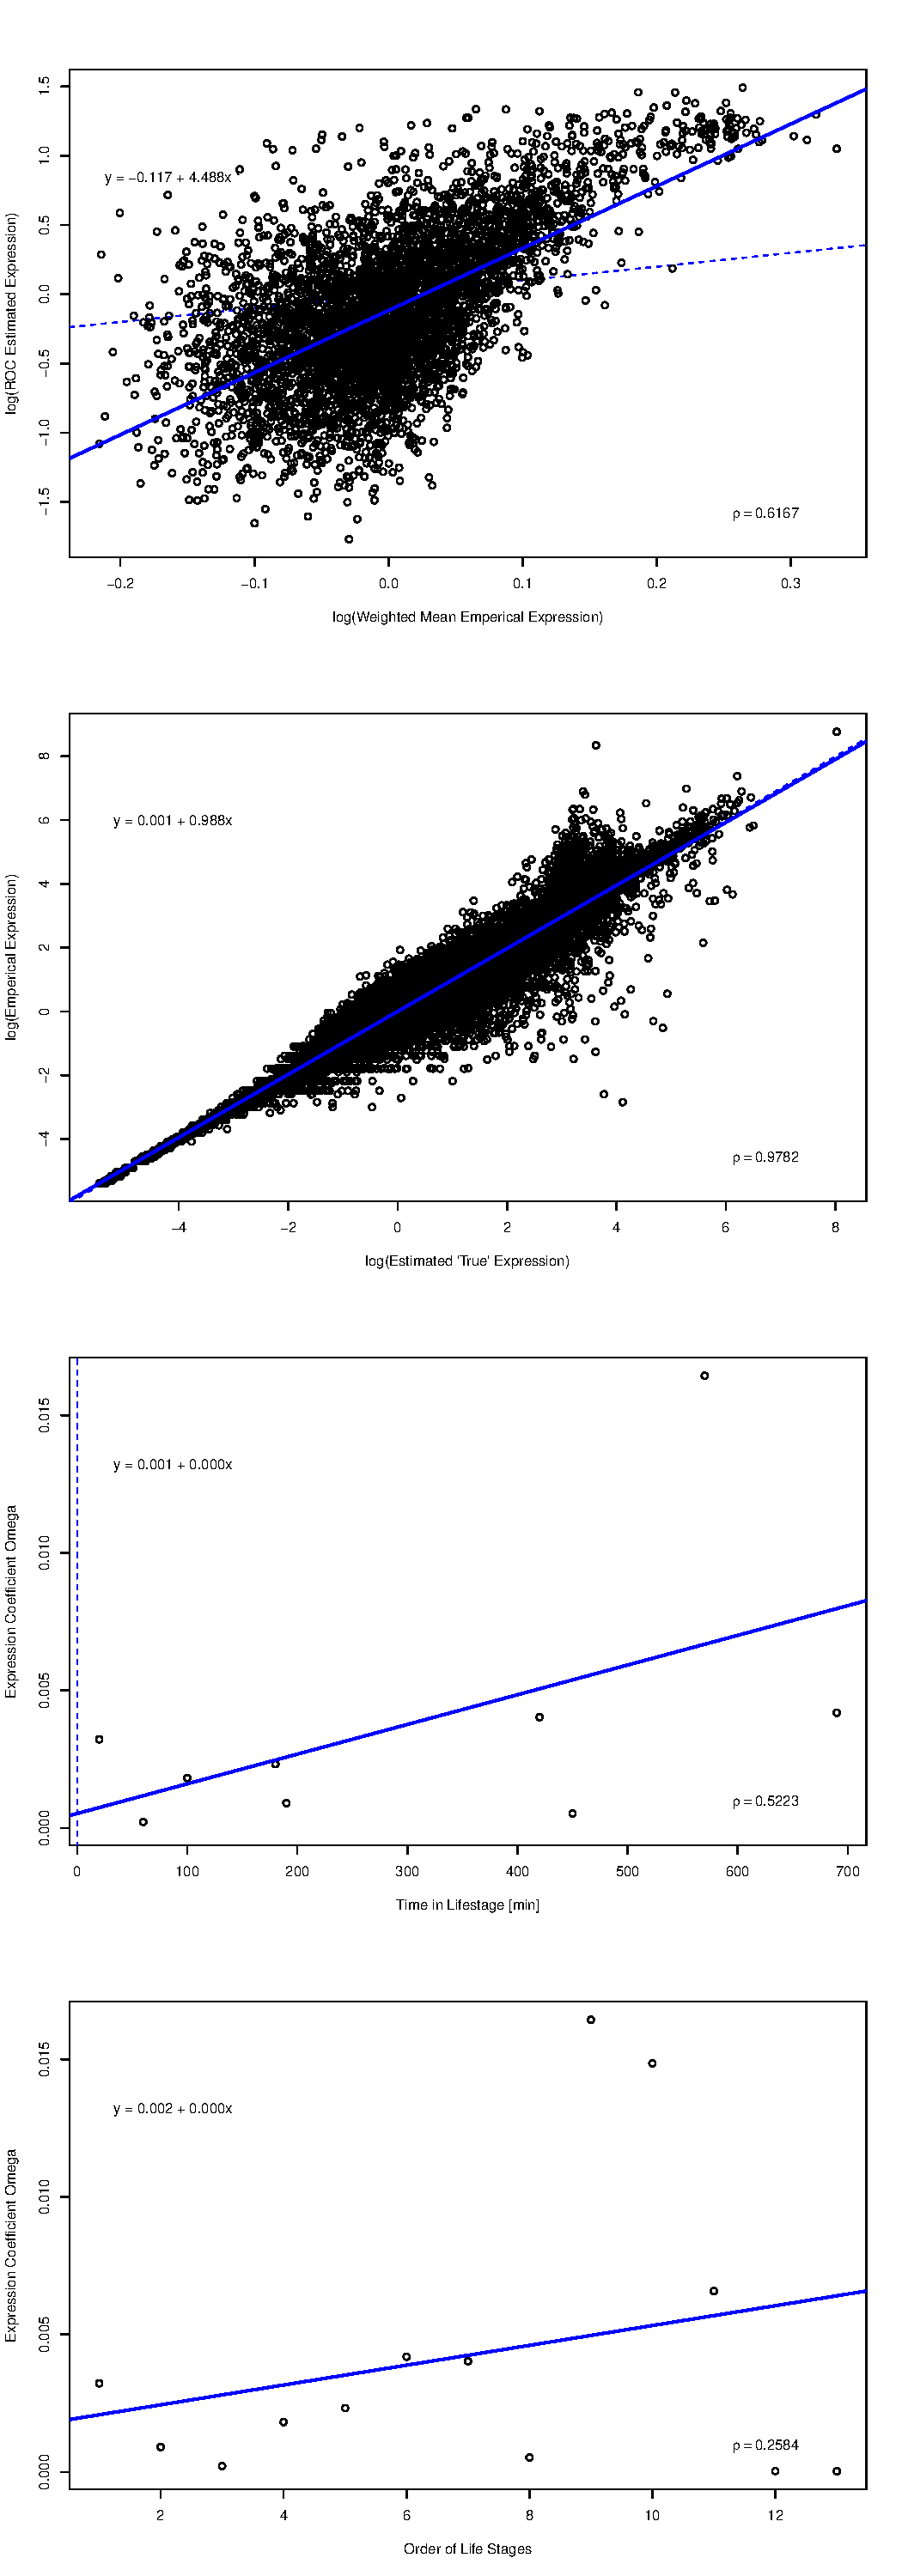
\includegraphics[scale=.45]{../C_Elegans/Lower_Hierarchy_With_Dauer_1/Plots/lower_hierarchy_with_dauer_original_model_celegans_weighted_expr_vector_beta_noise_fixed_sroc_withIntercept.pdf}
\end{center}
\caption{July 27th Graphs From Lower Hierarchy With Dauer Model Run}
\end{figure}

\begin{itemize}
\item **** Need to figure out how to display all 5 of the graphs that are on each pdf by splitting them onto multiple pages so they are not too small to read.
\item The first graph for each set of Figures charts the log of the Roc Estimated Expression on the y-axis and the log of the Weighted Mean of the Observed data. *** Need to look at this
\item The second graph displays the log Empirical Expression--the observed data-- versus the log Estimated True Expression.
\item The third graph displays the Time in Lifestage plotted with the Expression Coefficients
\item The fourth graph displays the ordering of the life stages.
\item I put these expected life stage durations and orderings in the file
\item  \enquote{C\_Elegans/Data/Ordered.Time.Spent.Lifestages.Celeg\_1.csv}.
\item The fifth graph displays the original log Roc expression data plotted against the log Mean Empirical Expression.
\item TO DO: While I am gone, Cedric has asked me to read a paper and compare it to our method of estimating codon optimality.
\end{itemize}


\labday{2 August 2016}
\experiment{Optimal Codons}
\begin{itemize}
\item Over the weekend Cedric asked me to read \enquote{Codon usage in "Caenorhabditis elegans": delineation of translational selection and mutational biases} (Stenico, et. al. 1994) and to see how our estimates of codon optimality line up with the paper's. 
\item I wrote my findings up in a word document, but I can easily move them to latex if need be.
\item For now I will put the word document in the Optimal Codons file.
\item I talked to Cedric and realized that I should have looked at the ROC SEMPRR data on C. Elegans instead of Yeast.
\item I analyzed and compared the C. Elegans optimal codons from ROC and from the Stenico file and compiled a table.
\item Just about all of the optimal codons were agreed upon by the two papers with the exception of Ser2, Arg, and Ser4, which are very logically explainable.
\begin{itemize}
\item Ser2- Stenico found no optimal codon between these two because neither shows up very often in high bias genes.
\item Arg- the top two most optimal codons are very close at the max phi levels, so it is not surprising that Stenico found CGC to be more optimal (but both to be optimal) while ROC found CGT/CGU to be more optimal.
\end{itemize}
\item I emailed Cedric the table and my comparison.
\item I printed the paper Dr. Gilchrist sent me to read and will comb through it.
\item When I talked to him a minute ago he said to focus on the methods of analysis and try to glean which method better fits the data and which method allows us to make more biological inferences.
\end{itemize}

\experiment{C. Elegans}
\begin{itemize}
\item Somehow I saved a blank sheet when I could have sworn I input the data from the Higher hierarchy with Dauer run, so the first thing I am doing this morning is re-inputting that data and making sure I save the file correctly.
\item I need to write code to send the results to an excel file so that I do not have to take the time and so there will be no human error when transferring the results.
\item Also writing code to export a file containing the mean log likelihood.
\item Finished writing those two codes and put them in both the rcodes on github.
\item Now that I have a table with all of the information about the mean betas and the expected life lengths, I can work on the mathematical code for deriving insight from this data.
\item Just realized I missed one life stage before that I somehow deleted from the data Cedric originally sent me.
\item It is called Newly Molted Young Adult Hermaphrodite.
\item This life stage occurs for the first 24 hours after the L4 and is considered part of the adult stage.
\item I am going back to alter the code and data for both datasets to include this life stage.
\item Changed the data and code and am re-running both datasets under the model.
\item I ran the lower hierarchy model and will run the higher hierarchy model tonight.
\item TO DO
\begin{itemize}
\item Add the newest data and figures to these notes and to the github.
\item Adjust the exported data's column names!
\item Talk to Gilchrist again about the Undergraduate Research Conference because I do not know if I can do it over fall break.
\end{itemize}
\end{itemize}

\end{document}